\section{Introduction}
\label{sec:intro}

Spiking neural networks (SNNs) are attractive for event-driven and low-power
inference, but modern visual recognition increasingly depends on Transformer
attention. Directly translating dense softmax attention into spikes is
difficult: attention weights depend on continuous query--key scores and on
row-wise normalization over all tokens. Recent spiking Transformers therefore
often redesign attention rather than convert standard attention literally.

QKFormer~\cite{zhou2024qkformer} is a strong example of this design direction.
Its spike-form Q-K attention uses binary vectors to model token or channel
importance and obtains a hierarchical spiking Transformer. This design raises a
different question from standard ANN-to-SNN conversion: if Q/K spike vectors
are already binary, can they form a useful discrete address space for lookup
modules?

This paper studies that question through QK-LUTFormer. We do not claim a pure
LUT hardware replacement for the full QKFormer block. Instead, we build a
diagnostic and adapter pipeline that asks whether Q/K binary addresses explain
attention-module responses better than non-address controls. To address the
obvious dimensionality concern of direct full-vector lookup, we additionally
evaluate two scalable lookup mechanisms: a support-aware hierarchy that makes
misses explicit, and a subspace-decoupled residual LUT that composes smaller
token/channel, Q/gate, and K subtables instead of materializing a monolithic
full-address table. For downstream utility, we additionally use frozen-backbone
residual LUT adapter probes with classification, baseline-logit distillation,
and local response constraints; these probes test whether the reconstruction
signal transfers to accuracy, rather than defining the main claim.

Our experiments show a clear separation between local response structure and
downstream classification. Correct compact addresses consistently reconstruct
held-out responses better than token/channel and shuffled controls across
datasets, checkpoints, time steps, and calibration budgets. Support-aware
backoff makes misses observable, while subspace decomposition preserves most of
the full-address gain below a fixed entry budget. Classification is evaluated
through a separate frozen-backbone gate, so local reconstruction is never
silently promoted into an accuracy claim.

\begin{figure*}[t]
  \centering
  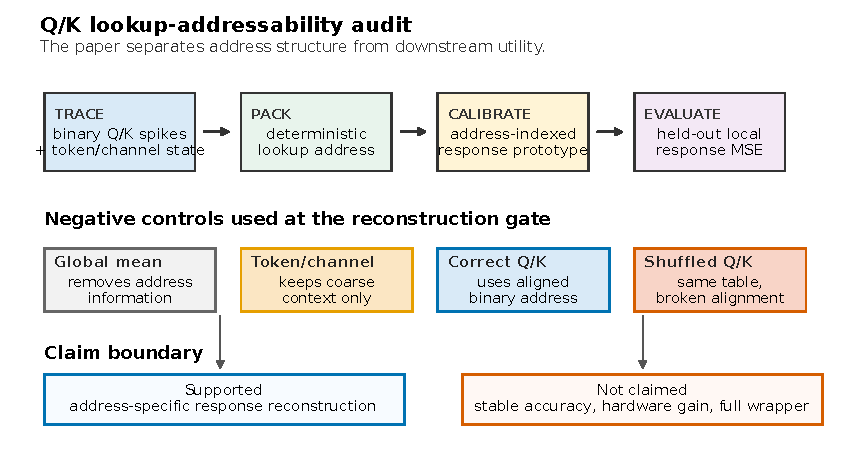
\includegraphics[width=\textwidth]{figures/fig1_audit_overview.pdf}
  \caption{Overview of the Q/K lookup-addressability audit. Binary Q/K states
  and token/channel context are packed into deterministic lookup addresses,
  calibrated against local module responses, and evaluated under four controls:
  global mean, coarse token/channel lookup, correct Q/K address lookup, and
  shuffled-address lookup. The audit separates supported response-structure
  evidence from unsupported downstream and hardware claims.}
  \label{fig:audit-overview}
\end{figure*}

Our contributions are:
\begin{itemize}
  \item We define code-faithful compact Q/K addresses for QKFormer and a
  negative-controlled audit of occupancy, conditional variance, and held-out
  response reconstruction. The audit replicates across CIFAR-10/CIFAR-100,
  time steps, calibration seeds, and independent checkpoints.
  \item We introduce support-aware hierarchical backoff and a
  subspace-decoupled QK-LUT. The latter replaces product-size lookup with a sum
  of semantic subtables and passes a predeclared 25\% supported-entry gate.
  \item We separate reconstruction from downstream utility through a registered
  frozen-backbone accuracy gate with global, token/channel, and shuffled
  controls, and explicitly bound claims that are not supported by that gate.
\end{itemize}
